\documentclass[a4paper,12pt,titlepage]{scrartcl}
\usepackage{palatino}
\usepackage{graphicx}
\usepackage{float}
\usepackage{amsmath}
\usepackage{caption}
\usepackage{subcaption}
\usepackage[margin=1.5cm,includefoot]{geometry}
\usepackage[utf8]{inputenc}
\usepackage{hyperref}
\usepackage{url}
\usepackage{listings}
\usepackage{xcolor}
%\usepackage{amsart}


\renewcommand*{\familydefault}{\sfdefault}

\usepackage[portuguese]{babel}



\begin{document}

\title{RFID - Radio Frequency Identification}
\subtitle{Aplicações em Integração de Dados}
\author{Victor São Paulo Ruela \\ Igor da Luz Pinheiro \\ \textbf{Universidade Federal de Minas Gerais}}
\date{\today}

\maketitle

\tableofcontents
\newpage 
\listoffigures

\listoftables
\newpage

\section*{Resumo}

%begin{document}

A tecnologia RFID (Radio Frequency Identification - identificador por rádiofrequência) designa um conjunto de tecnologias que utilizam a frequência de rádio para captura de dados de forma automática, por meio de um dispositivo eletrônico conhecido com tag RFID. Ele envia um sinal de radiofrequência para dispositivos leitores que captam estas informações. A integração dos dados RFID com o restante do sistema de gestão passa a ser então uma tarefa essencial para que possamos retirar informações valiosas destes dados. O objetivo deste trabalho é apresentar a descrição e exemplos de aplicação da tecnologia RFID, focados em aspectos relacionados à integração de dados. Nele serão explicados os elementos básicos de hardware e software presentes em todo sistema RFID, uma breve descrição sobra o histórico de adoção do RFID, uma introdução à norma EPCGlobal e alguns estudos de casos, focados nas soluções implementadas na integração dos dados.



%end{document}

\smallskip
\noindent \textbf{Palavras-Chave.} \textit{RFID, EPCGlobal, Integração de Dados, Middleware, Tags	}

\newpage

\section{Introdução}
\documentclass[a4paper,12pt,titlepage]{article}
\usepackage{palatino}
\usepackage{graphicx}
\usepackage{float}
\usepackage{amsmath}
\usepackage{caption}
\usepackage{subcaption}
\usepackage[margin=1.5cm,includefoot]{geometry}
\usepackage[utf8]{inputenc}
\usepackage{hyperref}
\usepackage{url}
\usepackage{listings}
\usepackage{xcolor}


\renewcommand*{\familydefault}{\sfdefault}

\usepackage[portuguese]{babel}

\begin{document}

	
	RFID, \textit{Radio Frequency Identification}, é uma tecnologia que está em crescente uso e discusssão atualmente, devido às suas possíveis aplicações e os benefícios que sua utilização propiciam. Seu principal uso é no monitoramento de ativos, permitindo conhecer toda a trajetória de um produto, desde o início da cadeia produtiva até o consumidor final. Avanços tecnológicos na fabricação de semicondutores permitiram tanto a redução do custo quanto a do tamanho dos componentes. Antes, as tags eram do tamanho de um forno-microondas e os leitroes construídos com antenas gigantescas. Hoje em dia, podemos encontrar leitores do tamanho de um moeda, e tags do tamanho de um grão de arroz, alavancando ainda mais a adoção da tecnologia RFID. Qualquer sistema de identificação no qual um dispostivo eletrônico usa radio frequência para o variações no campo magnético para comunicar e está anexado a um item, é definido como um RFID.
	
	Os dois principais componentes deste tipo de sistema são a \textit{Tag}, a qual é o dispositivo de identificação anexado ao item que desejamos monitorar, e o \textit{Leitor}, que é o dispositivo responsável por reconhecer as Tags e ler a informação contida nelas. O leitor pode então informar outros sistemas sobre a presença das tags, através de um \textit{RFID Middleware}. Este é um software que fornece a interface entre os leitores e o restante do sistema de informação. Na figura a seguir, podemos ver o sistema em questão:
	
	\begin{figure}[h!]
		\centering
		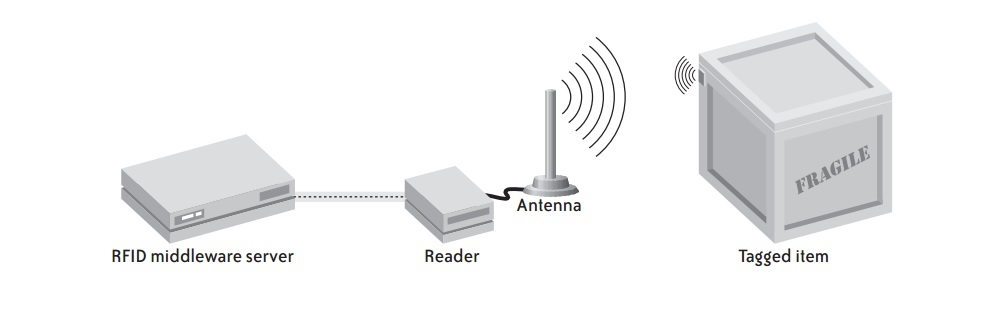
\includegraphics[width=0.6\linewidth]{rfidsys2}
		\caption{Sistema RFID típico, retirado de \cite{rfidbook}}
		\label{fig:rfidsys}
	\end{figure}
	
	Alguns dos benefícios do RFID são resumidos abaixo:
	\begin{itemize}
		\item Não há necessidade de alinhamento dos itens para leitura;
		\item Alta velocidade de inventário, pois vários itens podem ser lidos simultaneamente;
		\item Capacidade de identificar unicamente bilhões de itens;
		\item Variedade na forma das tags;
		\item Reusabilidade de tags.
	\end{itemize}
	
	\section{Evolução na adoção do RFID}
	De acordo com \cite{rfidbook}, podemos dividir o progresso de adoção do RFID em 5 períodos: \textit{Proprietary era}, \textit{Compliance era}, \textit{RFID-enable Enterprise era}, \textit{RFID-enable Industies era} e \textit{Internet of Things era}. A figura [\ref{fig:rfideras}] mostra quando algumas funções do RFID começaram ou vão começar a existir.
	
	\begin{figure}[h!]
		\centering
		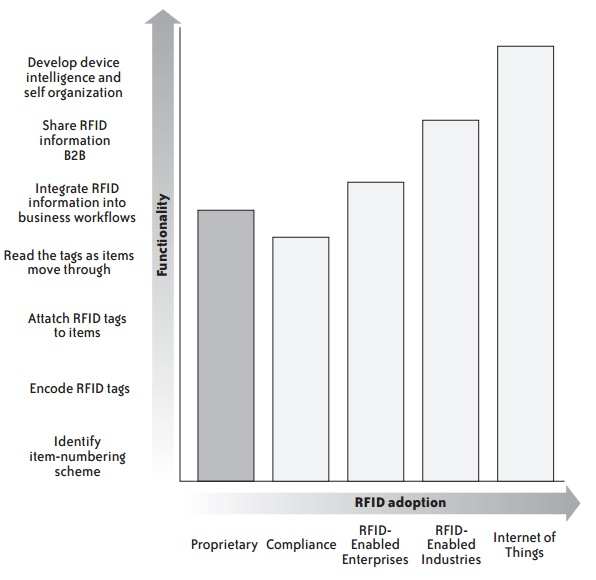
\includegraphics[width=0.6\linewidth]{rfideras}
		\caption{Evolução do RFID, retirado de \cite{rfidbook}}
		\label{fig:rfideras}
	\end{figure}
	
	No início (\textit{Proprietary era}), o RFID era usado para monitorar tipos particulares de itens e esta informação permanecia dentro das organizações que utilizavam o sistema. Isso fazia com que os sistemas fosse bastante específicos, dificultando bastante a comunicação entre parceiros de negócios. Alguns dos itens monitorados eram carros de trem, chassis de automóveis e gado leiteiro. Nesta época as tags ainda eram caras, logo estas eram reutilizadas sempre que possível. 
	
	Na \textit{Compliance era}, que representa o período atual, as empressas utilizam o RFID principalmente para garantir a interoperabilidade entre parceiros de negócios e agências regulatórias, não usando frequentemente os dados RFID para, por exemplo, aperfeiçoar alguns processos e melhorar a produtividade. A escassez de padrões e a falta de confiabilidade das novas tecnologias, impedem que as taga funcionem tão bem na prática como na época anterior.
	
	No futuro, teremos a \textit{The RFID-Enabled Enterprise era}, na qual as empresas começarão a utilizar as informações coletadas do RFID para o aprimoramento dos próprios processos. Isso será alcançado com a estabilização dos padrões e queda significativa dos custos. As empresas passarão a monitorar itens individuais ao invés de unidades de transporte, permitindo a coleta de mais informações sobre o processo. Entretanto, mesmo com a larga adoção interna do RFID, as empresas ainda precisam desenvolver os padrões necessários para permitir a troca de informações entre elas. 
	
	Em seguida teremos a \textit{The RFID-Enabled Industries era}, onde o uso de padrões RFID, redes de informação RFID, acordos de negócios e políticas de segurança e privacidade permitirão que empresas e cadeias de suprimentos troquem dados de forma segura e confiável entre si. Isso permitirá a descoberta de novas informações através do estudo  do grande volume de dados que estará disponível.   
	   
	Por fim, teremos a \textit{The Internet of Things era} que é atualmente uma previsão, na qual a ubiquidade da tecnologia RFID mudará a forma como vemos a relação entre informação, objetos físicos e localização. Por exemplo, a geladeira de nossa casa estará conectada à Internet e será capaz de ler a data de validade dos alimentos presentes e nos informar se algum deles já venceu. Além disso, ela poderá checar se algum produto está faltando e automaticamente realizar o pedido deste junto ao supermercado.
	
	A forma e velocidade com que os diversos tipos de usuários passarão por essas épocas não será feita de maneira uniforme. Atualmente, existem usuários que ainda estão na \textit{Proprietary era}, enquanto outros já estão começando a aplicar os conceitos da \textit{RFID-enabled Industries e Internet of Things}. Em algumas áreas, o RFID ainda nem começou a ser implementado.
	
	
	
	
	\newpage
	 \bibliographystyle{plain}
	 \nocite{*}
	 \bibliography{biblio_doc}
	 


\end{document}
\newpage

\section{Integração de Dados e RFID}


\subsection{Introdução}
		Com o avanço da tecnologia RFID e o crescente interesse popular e industrial por esta tecnologia, a área de TI tem sido desafiada a criar recursos que permitam a interface e integração com sistemas RFID. Cada tag em um sistema RFID possui uma identificação única (UID) e os que possuem memória são capazes de gravar informações sob demanda.
	
		Devido a popularidade dos RFID, foram propostas muitas aplicações. Por meio do sinal sem fio de curta distância, usuários de uma tag RFID podem ser monitorados dentro de uma área específica. Assim, sistemas RFID são normalmente utilizados para identificação de um hardware ou objeto em muitas aplicações. Muitas dessas aplicações são baseadas em ambientes internos ou pequenas áreas de serviço independentes do sistema utilizado.
	
		Aplicações RFID vão além de códigos de barra ou banco de dados portáteis. RFID pode ser utilizado para a Segurança da Cadeia de Suprimentos (SCS) e gestão da vida útil de equipamentos ou alimentos. Como exemplo podemos citar o envio de toneladas de rações do Exército dos Estados Unidos para as tropas no Iraque e em outras localidades do mundo. Estas transferências são feitas por navios, que carregam milhares de contêiners padronizados. Como o Exército dos EUA faz para garantir que essa transferência foi esquecida, adulterada ou exposta a condições ambientais inapropriadas? Eles utilizam a tecnologia RFID integrada com sofisticados sensores para uma uma série de eventos ambientais, tais como: temperatura, radiação, luz, agentes químicos, agentes biológicos, choque, sensores de portas, entre outros. Se alguém esta fazendo algo com o carregamento de comida, ou se ela apenas fica quente por muito tempo, o Exército dos Estados Unidos conseguem saber onde e quando esse evento ocorreu. Esta é apenas uma aplicação entre tantas outras de tecnologia RFID em uma organização, no nosso exemplo, o Exército dos EUA. Atualmente a maior barreira para a implantação e adoção de sistemas RFID é a integração com sistemas legados.
		
		
		\begin{figure}[h!]
			\centering
				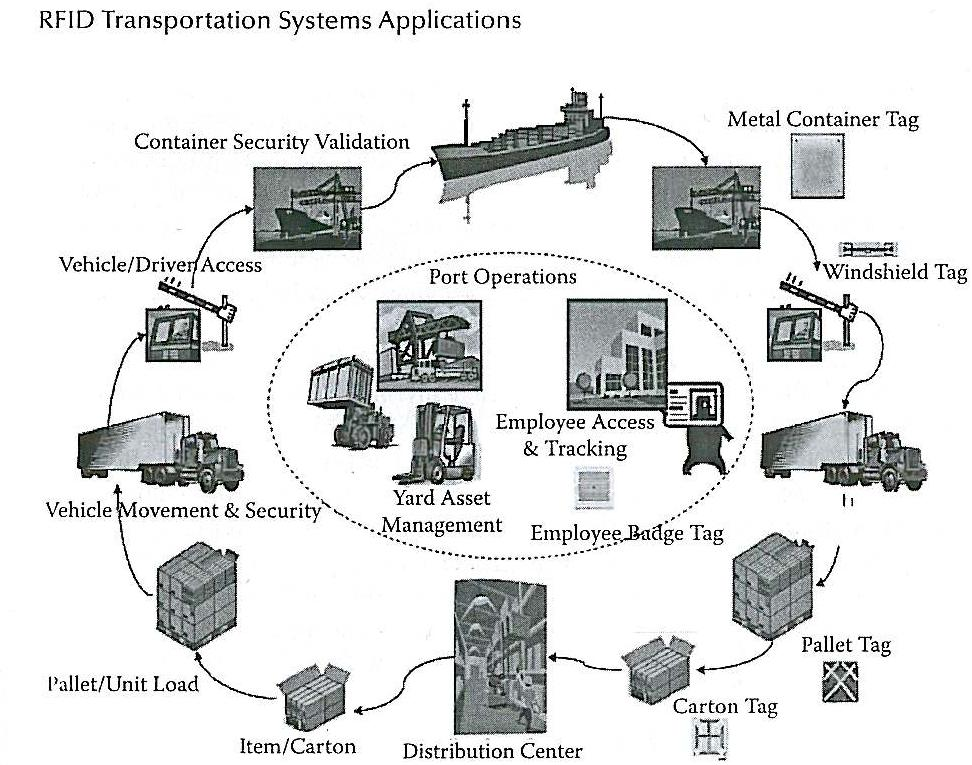
\includegraphics[width=0.7\linewidth]{Ex1SCS.jpg}
			\caption{Transporte de Alimentos monitorado por RFID}
			\label{fig:Ex1SCS}
		\end{figure}
		
	
	
		Alguns sistemas RFID foram propostos para serem utilizados em hospitais ou para cuidados da saúde[1]. Cada paciente recebe uma etiqueta (tag) RFID projetada. O paciente deverá usa-la constantemente, não importando o lugar nem o horário. Assim a localização e condições de saúde atuais do paciente poderão ser monitorados pelo hospital.
	
		Como RFID geralmente é utilizado para identificação, ele também pode ser utilizado em aplicações que usam criptografia de softwares como as identificações para proteger a propriedade intelectual de aplicativos ou arquivos. Algumas pesquisas mostram que o RFID pode ser incorporado em pequenos dispositivos. Os usuários do dispositivo podem conectar uma interface SD de leitor de cartão RFID. Dessa maneira os usuários poderão digitalizar e introduzir o RFID em todos os lugares. Uma vez que sistemas RFID fazem tratamento distintivo de um alvo individual, a caracterísitica única ou identificação RFID pode ser uma solução para a proteção da propriedade intelectual.
	
		Como se pode perceber esse conjunto de tecnologias baseadas em radiofrequência abriram uma ampla gama de possibilidades e oportunidades de forma direta e integrada para diferentes campos e áreas técnicas. Requisitos para efetiva implementação do sistema RFID exigem produtos específicos RFID, serviços e soluções de acordo com a escala e exigência do negócio.
		
		Dada a grande variedade de sistemas RFID, torna-se necessário o desenvolvimento de ferramentas de integração flexíveis, independentes de sistema operacional.
		
		
	
		
\subsection{Integração}
		O próprio leitor de RFID não pode lidar com a informação coletada de forma independente, tornando-se essencial a integração com outros sistemas ou ser agregado em aplicações existentes. Primeiramente, o designer do aplicativo tem que saber se a integração do aplicativo é baseada em software, hardware ou ambos. Se for um novo sistema, RFID poderá ser diretamente incorporado nele. No entanto, se a integração for com um sistema que ja existia, uma interface deverá ser decidida e definida.
		
		
\subsection{Vantagens da integração}
		Tecnologia RFID possui muitas características que a torna interessante e viável para integração com uma grande variedade de aplicações na industria, consumidores e comércio. Para integrar sistemas RFID eficientemente, é necessário a cooperação multidisciplinar de profissionais da área de TI, gestão de processos, projetistas de sistema, entre outros. Os RFIDs são mais ricos de informação do que os tradicionais códigos de barras. As etiquetas (ou tags) RFID geram valor ao produto pelas seguintes características:
		
		
		\begin{itemize}
			\item RFID não necessita de leitura visual, podendo realizar a leitura do objeto de dentro da caixa;
			\item Recurso de leitura/escrita criptografadas com usuários requeridos no armazenamento de dados;
			\item Monitoramento em tempo real por meio da internet/intranet para controle de estoques, redução de desperdícios e integração mais apertada da cadeia de suprimentos;
			\item Identificação automática por meio de redes sem fio;
			\item Podem sobreviver vários anos em ambientes hostis;
			\item Vários tipos de leitores de tags RFID estão disponíveis, como antenas inteligentes e impressoras portáteis.
		\end{itemize}
		
	
\subsubsection{Processo de Integração RFID}
Integração de sistemas RFID eficiênte exige conhecimentos abrangentes e a compreensão de diferentes sistemas. Para integrar funções RFID dentro de um sistema com outras tecnologias, como scan, controle e tecnologia da informação exige conhecimento e experiência com integração e hardware.


\begin{figure}[h!]
	\centering
		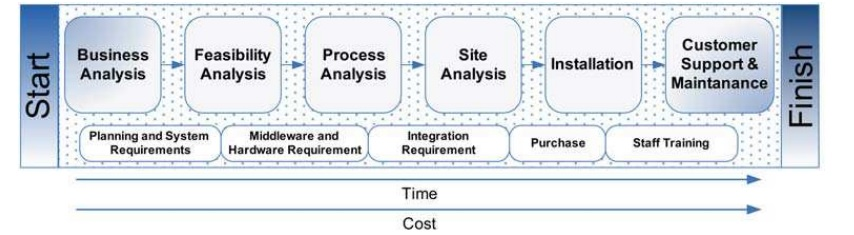
\includegraphics[width=0.7\linewidth]{etapas_integracao.jpg}
	\caption{Etapas para o projeto de Integração de Sistemas RFID.}
	\label{fig:etapas_integracao}
\end{figure}


		Cada projeto de negócio tem seus próprios requisitos e obstáculos técnicos que exige personalização de sistemas RFID. Deve-se, primeiramente fazer uma análise de viabilidade do meio. Para resolver eventuais problemas é aconselhado fazer a instalação de RFID em etapas. No processo de implementação cada etapa poderá ser revisada. Em alguns ambientes, leitores RFID móveis podem ser utilizados para aumentar ou substituir modelos estacionários.
		Para aumentar a confiabilidade deve-se fazer um planejamento e implementação de reconfigurações, gravação otimizada, segurança e autentificação.
		

\subsubsection{Componentes para Integração com Sistemas RFID}
Além dos componentes básicos de um sistema RFID, como tag, leitor e middleware, outros componentes também devem se levados em consideração para ser feita a integração. A figura abaixo apresenta o esquemático dos componentes necessários para a integração:


\begin{figure}[h!]
	\centering
		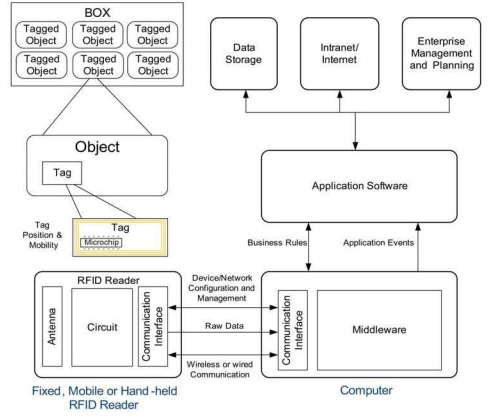
\includegraphics[width=0.5\linewidth]{componente integracao.jpg}
	\caption{Componentes para Integração de RFID.}
	\label{fig:componente integracao}
\end{figure}


\subsubsection{Posição e Mobilidade da Tag}
Este fator é necessário ser levado em consideração para obter uma melhor performance do sistema. Quando a tag ou o leitor estão se movendo, trata-se de mobilidade. Para poder garantir a identificação da tag, a velocidade do movimento deve ser levada em consideração.
		
		A decisão da posição da tag é crítico para tags passivas. Essa escolha deve levar em consideração a Potência Efetiva Radiada, que pode ter efeitos como ressônancia do sinal e morte do sinal.
		
		
\subsubsection{Módulos de Comunicação}
Diferentes formas de conexão podem ser utilizados, com ou sem fio. Padrões e normas variados podem ser utilizados, dependendo  do tipo de comunicação: com/sem fio, tipo de conector, custo, alcance, requisitos de segurança de aplicativos, entre outros.


\subsubsection{Aplicativos de Software para Integração de Sistemas}
Aplicativos de software executam em computadores comuns ou servidores e que comunicam com o middleware, controladores e dados de equipamentos de automação podendo realizar o controle das operações do Workflow.

		Os sistemas RFID exigem software que gerencia dispositivos, dados, rede e processos para permitir um fluxo contínuo de informação, alertas e respostas em tempo real.

		
\subsubsection{Servidor para Gravação de Dados}
	Usando uma apropriada infra-estrutura de rede, os dados obtidos de middleware podem ser gravadas e utilizadas para o desenvolvimento, implantação e manutenção de soluções produtivas. O servidor central executa aplicação de banco de dados com funções que incluem correspondência, rastreamento e armazenamento.


\subsubsection{Integração de RFID com simples Circuito}
Muitos sistemas de controle mecânico simples tem seu hardware baseado em projeto de circuitos. De acordo com a exigência ou ação da máquina, algumas ações mecânicas são acionadas quando recebem um sinal de On/Off. O leitor do sistema RFID atua como um fio elétrico para a transmissão de sinal para o circuito simples.


		\begin{figure}[h!]
			\centering
				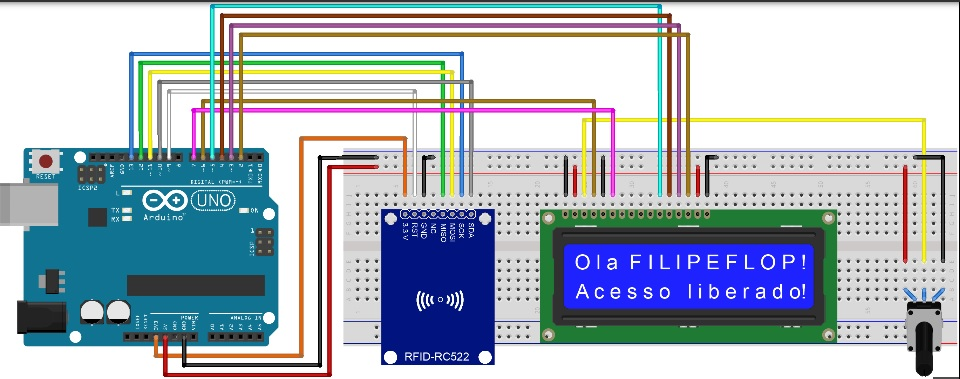
\includegraphics[width=0.7\linewidth]{mosfet_rfid.jpg}
			\caption{Exemplo de Circuito integrado a RFID.}
			\label{fig:mosfet_rfid}
		\end{figure}
		

		Neste tipo de integração, o sistema RFID funciona como um emissor de sinais. Quando o leitor de RFID induz as tags RFID, o leitor verifica se o tag RFID induzida é a tag pré-definida ( por exemplo, como válida) ou não. Se a tag induzida for uma pré-definida, o leitor envia o sinal de controle para acionar o hardware ou ação mecânica tal como abrir a porta de bloqueio. Dessa forma o sistema integrado vai agir com base na decisão do sistema RFID.
		
		
\subsubsection{Porta Serial RS-232}
O RS-232 consiste de dois dispositivos: DTE e DCE. Ao enviar sinal de controle, os dispositivos podem comunicar entre si via cabo RS-232. De acordo com o padrão de comunicação RS-232, o leitor do RFID pode enviar comandos pré-definidos através de RS-232 para acionar uma máquina ou sistema; ou então enviar um sinal emulado como comando para acionar os sistemas. Neste tipo de integração o RFID, pode exercer as seguintes funções: servir como um fio elétrico que aciona sistemas ou ser atuar como uma unidade computacional simples (IC chip) para o controle da porta serial e o comando de ordenação.


\subsubsection{USB e Acesso à internet}
Dependendo do hardware do computador, o leitor de RFID pode se conectar ao computador via porta USB ou conexão RJ45 Internet. Quando se conecta via USB, a informação da tag RFID pode ser transmitida para o PC diretamente. As aplicações que recebem informações do leitor RFID podem melhorar as funções ou capacidades dos serviços. O sinal de controle, a função de execução, ou ainda a gestão da informação podem ser feitos pelos aplicativos.

		Se a comunicação é através da internet, o leitor de RFID tem, pelo menos, o componente de rede e uma unidade de processamento central de informações suficientes para a computação. O sistema RFID funcionará como um dispositivo de rede pertencente a rede da plataforma, podendo agir de forma independente. O acesso pelo cabo de Internet é apenas para transmissão de dados e informações.
		
		Não importa se a comunicação é com base na porta USB ou pela conexão de rede, o sistema RFID tem apenas o papel de coleta informações.




\subsection{Considerações Finais}
Nesta seção foram vistos diversos exemplos de situações em que são ou podem ser empregados a integração de sistemas RFID. Também foram vistos os componentes necessários para permitir essa comunicação.
Por fim o capítulo apresentou diferentes conexões com fio entre o sistema RFID e um dispositivo, geralmente um computador.

		
	
\newpage

\section{Estudos de Caso}


%caso 1
\subsection{Autenticação de bebidas}
Este caso consiste da implementação de um sistema RFID pela fabricante de bebidas de Taiwan \textit{Taiwan Tobacco and Liquor Corp.} (TTL). O objetivo da adoção foi assegurar a autenticidade de seus produtos e rastrear as mercadorias pela cadeia de suprimentos. 
A empresa produz principalmente vinhos finos e bebidas de alto valor, portanto é de seu interesse garantir a autenticidade de seus produtos, principalmente no mercado da China.

Para desenvolver este sistema, a TTL decidiu trabalhar com a EPC Solutions Taiwan. A solução deveria ser capaz de todos os produtos em sua cadeia de suprimentos, passando pelo engarrafamento, embalagem e recebimento de mercadorias no centro de distruibuição (CD) na China.  Além disso, os clientes deveriam ser capazes de confirmar a autenticidade do produto através de um leitor portátil, o qual interrogaria o rótulo de cada garrafa.

Como a TTL deveria fornecer um leitor para cada revendedor, a escolha deste era um fator crucial projeto, pois era preciso um leitor que funcionasse bem e barato. Para isso, A EPC Solutions desenvolveu um leitor de baixo custo operando em 433 MHz capaz de ler as tags RFID passivas EPC Gen2 UHF escolhidas para a aplicação. 

\begin{figure}[h!]
\centering
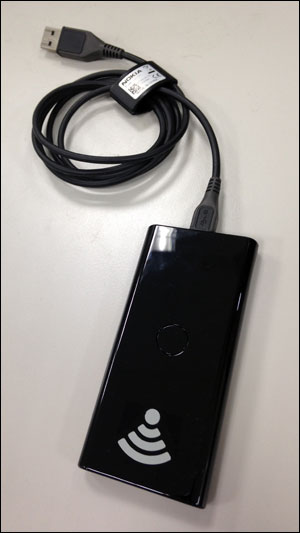
\includegraphics[width=0.2\linewidth]{leitor_ttl}
\caption{Leitor desenvolvido}
\label{fig:leitor_ttl}
\end{figure}
   
Nos armazéns, fábricas e centros de distribuição, foram instalados três leitores UHF 902-928 MHz para interrogar as tags. Escolheu-se um frequência de operação maior de forma a permitir a leitura a maiores distâncias.

Na estação de engarrafamentoe, as tags são afixadas no topo da garrafa através de um adesivo não removível, interrogadas automaticamente e seus dados são enviados a servidor back-end da TTL, onde o software relaciona o tipo de produto e lote com o número de identificação único da tag.

Ao chegar na estação de embalagem, os funcionários empacotam 6 garrafas em uma caixa e adicionam outra tag à esta caixa. Todas a 7 tags são lidas pelo próximo interrogador, o qual vincula as tags dos frascos à da embalagem.

Por fim, as caixas são carregadas em paletes e um leitor fixos lê as tags das garrafas e da caixa, relacionando essa informação com a etiqueta afixada no palete. Os paletes são então transferidos para o armazém, onde leitores fixos registram a chegada dos bens e funcionários com leitores de mão fazem verificações periódicas de inventário.

No momento da expedição, os bens passam por um portal leitor fixo que atualiza o software e indica que o palete foi enviado ao CD. No CD, leitores fixos foram instalados para indicar o recebimento do palete e equipamentos de mão são usados para controle de estoque. Os dados são então enviados ao servidor da TTL para atualização.

Nas lojas, os consumidores podem conectar o leitor \ref{fig:leitor_ttl} ao seu tablet ou smartphone e baixar o aplicativo da TTL para conseguir confirmar a autenticidade do produt através da leitura da tag do produto. Em cada leitura, um consulta é feita ao servidor da TTL, de forma a garantir esta procedência.

\subsection{title}


\subsection{title}

\newpage

\section{A Norma EPCGlobal}
\documentclass[a4paper,12pt,titlepage]{article}
\usepackage{palatino}
\usepackage{graphicx}
\usepackage{float}
\usepackage{amsmath}
\usepackage{caption}
\usepackage{subcaption}
\usepackage[margin=1.5cm,includefoot]{geometry}
\usepackage[utf8]{inputenc}
\usepackage{hyperref}
\usepackage{url}
\usepackage{listings}
\usepackage{xcolor}


\renewcommand*{\familydefault}{\sfdefault}
\usepackage[portuguese]{babel}


\begin{document}

\section{Introdução}	
	O uso da tecnologia RFID está em crescente expansão, principalmente em aplicações de Supply Chain Management (SCM), no qual saber a localização de cada item da cadeia produtiva é crucial para garantir maior eficácia e eficiência de todo um sistema. Devido essa crescente adoção do RFID, fica constatado que o surgimento de um conjunto de normas que visem à padronização das tecnlogias usadas seria algo natural de se acontecer. Imagine a situação em que uma grande empresa do setor de varejo se funda com outra do mesmo setor, sendo que ambas usam RFID para a localização dos produtos. Se, por exemplo, o formato das TAGs utlizadas pelas empresas forem diferentes, já teremos uma enorme dificuldade de integrar as informações oriundas de cada sistema. Para contornar esse tipo de problema, existe o \textbf{GS1}.
	
	O GS1 é uma organização internacional neutra e sem fins lucrativos, que desenvolve e mantém padrões para cadeias de demanda e suprimentos de diversos setores produtivos. Ele atua principalmente nas áreas de bens do consumo e varejo, saúde e transporte e logística. Algumas empresas que trabalham com o GS1 são: Carrefour, amazon, Google e Coca Cola. 	
	O GS1 foi fundado na década de 70 pelos líderes da indústria dos EUA, tendo com sua primeira atividade a criação do padrão de código de barras conhecido como \textbf{GS1 barcode}, o qual é largamente utilizado até hoje. Com os avanços da tecnologia e seu crescente uso, em 2004 o GS1 criou o primeiro padrão para o RFID.

	O padão GS1 é divido em três grupos: Identificar, Capturar e Compartilhar. 
	\begin{figure}[h!]
		\centering
		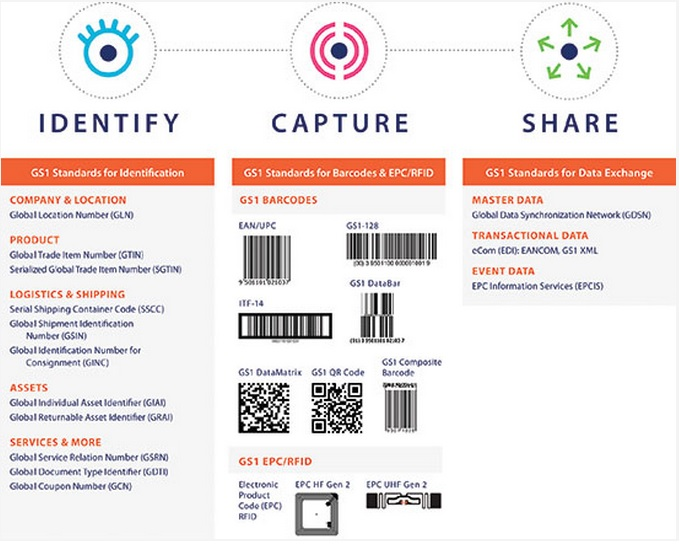
\includegraphics[width=0.7\linewidth]{gs1arch}
		\caption{Arquitetura do GS1}
		\label{fig:gs1arch}
	\end{figure}

	\paragraph{Identificar} Define códigos de identificação únicos que podem ser usados por um sistema de informação para se referir sem ambiguidade a qualquer tipo de produto.
	\paragraph{Capturar} Inclui definições de códigos de barra e RFID, além de especificar padrões para interfaces entre os elementos de software e hardware que se conectam às aplicações empresariais.
	\paragraph{Compartilhar} Define padrões para o formato dos dados trocados entre as aplicações e os clientes.     

	A norma voltada paraaplicações com RFID se enquadra no grupo "Capturar", e suas definições estão presentes no \textbf{EPCGlobal}.


\section{O padrão EPCGlobal}
	O padrão EPCglobal é uma iniciatia do GS1 para desevolver padrões voltados à indústria para o EPC, com o objetivo de dar suporte ao uso de RFID. Ele é divido em duas partes: \textbf{EPC/RFID Tags} e \textbf{EPCIS}. 
	
	O EPC (Electronic Product Code) é responsável por interligar o mundo do RFID com os códigos de barra do padrão GS1. Isso funciona da seguinte forma:
		\begin{figure}[h!]
			\centering
			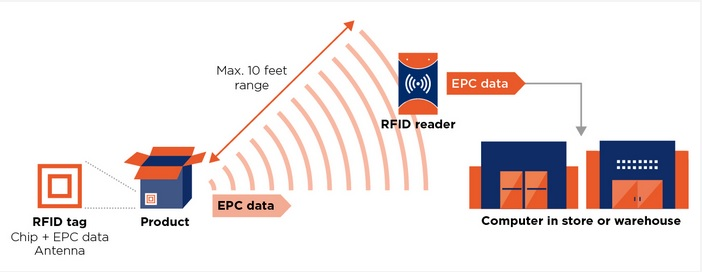
\includegraphics[width=0.5\linewidth]{epcrfid}
			\caption{Funcionamento do EPC}
			\label{fig:epcrfid}
		\end{figure}
	
	Cada produto contém um chip de memória contendo um EPC, o qual consiste de um número de série único. Em cada chip também há uma antena de rádio que transmite o EPC para um leitor RFID quando requisitado. Os dados capturados pelo leitor são então disponibilizados para os outros sistemas. A
	
	
	\begin{figure}[h!]
		\centering
		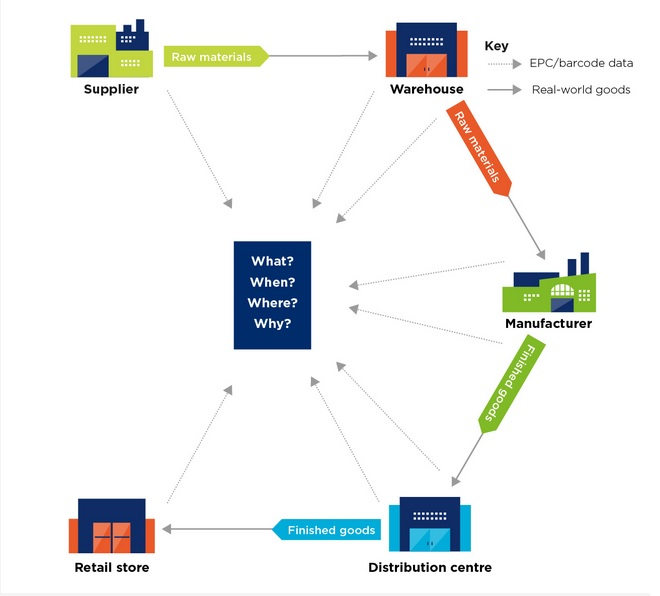
\includegraphics[width=0.5\linewidth]{epcis}
		\caption{Funcionamento do EPCIS}
		\label{fig:epcis}
	\end{figure}
	
	% Falar sobre o EPCIS
	O EPCIS (Electronic Product Code Information Services) é o padrão que habilita as empresas parceiras a compartilhar informações sobre o movimento físico e status dos produtos enquanto eles trafegam pela linha de suprimentos. Uma vez que os dados EPC são coletados, como na figura \ref{fig:epcrfid}, eles são disponibilizados à camada de negócios e todos que possuem acesso a este podem saber o histórico de movimento dos produtos. 
	
	\subsection{Arquitetura}

	O EPCGlobal define somente as interfaces, deixando as questões relativas à implementação sobre responsabilidade do usuário. Isso garante uma maior flexiblidade e alimenta o mercado de soluções em sistemas de informação para alcançar essa integração dos dados da cadeia produtiva. A figura \ref{fig:epcarc} apresenta um diagrama contendo a arquitetura básica de um sistema operando com a norma EPCGlobal.

	\begin{figure}[h!]
		\centering
		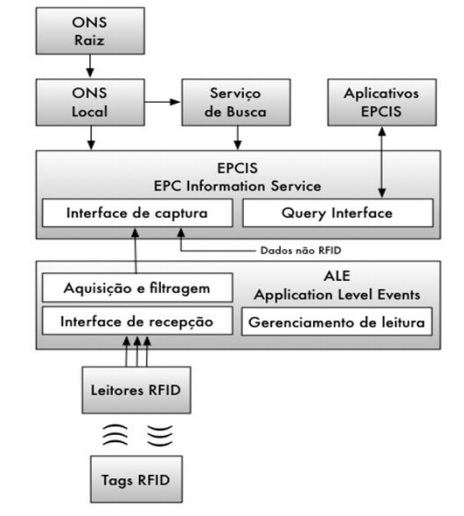
\includegraphics[width=0.5\linewidth]{epcarc}
		\caption{Arquitetura do EPCGlobal. Retirada de \cite{epcSobCug} }
		\label{fig:epcarc}
	\end{figure}
	
	A primeira camada contém os elementos necessários que permitem a identificação única de cada elemento da cadeia produtiva. Ela é composta pelo EPC, Tags e leitores RFID. 
	
	Entre os leitores RFID e as aplicações de captuda de dados está a interface ALE (Application Level Events). A ALE é uma camada de \textit{Middleware}, responsável por oferecer uma interface de alto-nível às aplicações capaz de agragar dados de diversos leitores, filtrá-los para remover redundâncias, como leituras múltiplas e não-desejadas e disponibilizá-los de maneira que as aplicações possam trabalhar mais facilmente com esses dados. Resumindo, a ALE é uma interface de pré-processamento de dados, que elimina a necessidade das aplicações de captura de dados lidarem com os aspectos de baixo nível da leitura de dados.
	
	Acima da ALE, temos o EPCIS. Esta é uma interface entre a captura de dados e as aplicações de nível empresarial. A troca de dados provenientes da ALE é feita através de mensagens XML padronizadas, tornando possível o uso do protocolo \textit{SOAP}. O compartilhamento destes dados para o público consumidor e/ou parceiros de negócios é definido pelas empresas, as quais decidem o grau com que elas irão disponiblizar essa informações. Este serviço é garantida pela \textit{Query Interface}, a qual integra os sistemas através de \textit{web services}, utilizando para isto os conceitos do \textit{SOA}. 
	
	Nas camadas mais superiores temos o Object Name Services (ONS), o qual é responsável por descobrir informações sobre um objeto com base no EPC. Para um dado EPC, a URL ou IP associado é pesquisado no banco de dados e os dados referentes àquele objeto podem ser econtrados e devolvidos à quem o requisitou. Ele funciona de maneira análoga a um servidor DNS, o qual traduz domínios em endereços IP.
	
\newpage

\bibliographystyle{plain}
\nocite{*}
\bibliography{biblio_doc}

		
\end{document}
\newpage

\section{Conclusão}


%\begin{document}

Neste trabalho apresentamos a descrição da tecnologia RFID, explicando como funcionam os seus diferentes componentes: tags, leitores e \textit{Middleware}. Do ponto de vista de integração de dados, o \textit{Middleware} é o elemento mais importante, uma vez que ele é responsável pela interface entre os sistemas físicos de acquisição de dados RFID e os outros sistemas empresariais. O RFID é usado principalmente para a localização e monitoramento de ativos, onde precisamos saber por onde e quando passou cada elemento da cadeia produtiva. Por causa disso, esta é uma tecnlogia que está em constante aprimoramento e crescimento no número de empresas que a adotam.

Através dos estudos de casos, foi possível ver na prática como os conceitos explicados anteriormente são aplicados, mostrando os desafios e dificuldades encontradas na implementação deste tipo de sistema. Os mesmos problemas decorrentes da heterogeneidade dos elementos da arquitetura do sistema puderam ser vistos nestas aplicações práticas. Para tentar contorná-los, forma criados diversas normas e entre elas podemos citar a EPCGlobal. Ela define tanto os aspectos de hardware quanto os da arquitetura, de forma melhorar visivelmente a eficiência de todo do sistema. Isso foi comprovado pelo estudo de caso da norma apresentado.

Logo, podemos concluir que o trabalho realizado cumpriu os objetivos propostos, apresentando uma boa descrição da tecnologia RFID, focada nos aspectos de integração de dados.  

 
%\end{document}

\newpage
\bibliographystyle{plain}
\nocite{*}
\bibliography{biblio_doc}



\end{document}